%% ----------------------------------------------------------------
%% Thesis.tex -- MAIN FILE (the one that you compile with LaTeX)
%% ---------------------------------------------------------------- 

% Set up the document
\documentclass[a4paper, 11pt, oneside]{Thesis}  % Use the "Thesis" style, based on the ECS Thesis style by Steve Gunn
\graphicspath{{./Figures/}}  % Location of the graphics files (set up for graphics to be in PDF format)
\DeclareGraphicsExtensions{.pdf,.png,.jpg}

% Include any extra LaTeX packages required
\usepackage[square, numbers, comma, sort&compress]{natbib}  % Use the "Natbib" style for the references in the Bibliography
\usepackage{verbatim}  % Needed for the "comment" environment to make LaTeX comments
% \usepackage{vector}  % Allows "\bvec{}" and "\buvec{}" for "blackboard" style bold vectors in maths
\hypersetup{urlcolor=blue, colorlinks=true}  % Colours hyperlinks in blue, but this can be distracting if there are many links.

%% ----------------------------------------------------------------
\begin{document}
\frontmatter      % Begin Roman style (i, ii, iii, iv...) page numbering

% Set up the Title Page
\title  {Hoe realiseren we een ontwikkel omgeving waarin niet-programmeurs, zoals 3D artiesten en level designers, efficiënt unieke virtual reality ervaring kunnen creëren in Unreal Engine 4}
\authors  {\texorpdfstring
            {\href{marktarts93@gmail.com}{Mark Arts}}
            {Mark Arts}
            }
\addresses  {\groupname\\\deptname\\\univname}  % Do not change this here, instead these must be set in the "Thesis.cls" file, please look through it instead
\date       {\today}
\subject    {Virtual Reality}
\keywords   {}

\maketitle
%% ----------------------------------------------------------------

\setstretch{1.3}  % It is better to have smaller font and larger line spacing than the other way round

% Define the page headers using the FancyHdr package and set up for one-sided printing
\fancyhead{}  % Clears all page headers and footers
\rhead{\thepage}  % Sets the right side header to show the page number
\lhead{}  % Clears the left side page header

\pagestyle{fancy}  % Finally, use the "fancy" page style to implement the FancyHdr headers

%% ----------------------------------------------------------------
% The "Funny Quote Page"
\pagestyle{empty}  % No headers or footers for the following pages

\null\vfill
% Now comes the "Funny Quote", written in italics
\textit{``I choose a lazy person to do a hard job. Because a lazy person will find an easy way to do it.''}

\begin{flushright}
Bill Gates
\end{flushright}

\vfill\vfill\vfill\vfill\vfill\vfill\null
\clearpage  % Funny Quote page ended, start a new page
%% ----------------------------------------------------------------

% The Abstract Page
\addtotoc{Abstract}  % Add the "Abstract" page entry to the Contents
\abstract{
\addtocontents{toc}{\vspace{1em}}  % Add a gap in the Contents, for aesthetics

The Thesis Abstract is written here (and usually kept to just this page). The page is kept centered vertically so can expand into the blank space above the title too\ldots

}

\clearpage  % Abstract ended, start a new page
%% ----------------------------------------------------------------

\setstretch{1.3}  % Reset the line-spacing to 1.3 for body text (if it has changed)

% The Acknowledgements page, for thanking everyone
% \acknowledgements{
% \addtocontents{toc}{\vspace{1em}}  % Add a gap in the Contents, for aesthetics

% Als eerste wil ik DPI bedanken voor het mogelijk maken en het faciliteren van deze scriptie. Extra dank gaat naar Boy .... die ons met enthousiasme en vertrouwen begeleid heeft.

% Naast DPI ben ik dankbaar voor het zelfde enthousiasme en vertrouwen van Emiel Bakker onze afstudeer begeleider vanuit het HRO.

% Randy Dijkstra, die zijn scriptie aan de andere kant van mijn bureau schreef, wil ik bedanken voor zijn vriendschap. Zonder jou had ik aanzienlijk minder motivatie gehad om een uitdagend onderwerp te kiezen, laat staan het succesvol afronden ervan.

% Als laatste bedank ik mijn ouders voor het dak boven mijn hoofd, mijn avondeten, het wassen, het opruimen en natuurlijk voor alle mogelijkheden die ze mij gegeven hebben om mijzelf te ontwikkelen. 

% }
% \clearpage  % End of the Acknowledgements
%% ----------------------------------------------------------------

\pagestyle{fancy}  %The page style headers have been "empty" all this time, now use the "fancy" headers as defined before to bring them back


%% ----------------------------------------------------------------
\lhead{\emph{Contents}}  % Set the left side page header to "Contents"
\tableofcontents  % Write out the Table of Contents

%% ----------------------------------------------------------------
%\lhead{\emph{List of Figures}}  % Set the left side page header to "List if Figures"
%\listoffigures  % Write out the List of Figures

%% ----------------------------------------------------------------
%\lhead{\emph{List of Tables}}  % Set the left side page header to "List of Tables"
%\listoftables  % Write out the List of Tables

%% ----------------------------------------------------------------
\setstretch{1.5}  % Set the line spacing to 1.5, this makes the following tables easier to read
\clearpage  % Start a new page
\lhead{\emph{Abbreviations}}  % Set the left side page header to "Abbreviations"
\listofsymbols{ll}  % Include a list of Abbreviations (a table of two columns)
{
% \textbf{Acronym} & \textbf{W}hat (it) \textbf{S}tands \textbf{F}or \\
\textbf{HRO} & \textbf{H}ogeschool \textbf{RO}tterdam \\
\textbf{VS} & \textbf{V}isual \textbf{S}cripting \\
}

%% ----------------------------------------------------------------
% End of the pre-able, contents and lists of things
% Begin the Dedication page

% \setstretch{1.3}  % Return the line spacing back to 1.3

% \pagestyle{empty}  % Page style needs to be empty for this page
% \dedicatory{Voor all mijn vrienden die om onverklaarbare redenen graag met mij omgaan}

% \addtocontents{toc}{\vspace{2em}}  % Add a gap in the Contents, for aesthetics


%% ----------------------------------------------------------------
\mainmatter	  % Begin normal, numeric (1,2,3...) page numbering
\pagestyle{fancy}  % Return the page headers back to the "fancy" style

% Include the chapters of the thesis, as separate files
% Just uncomment the lines as you write the chapters

%!TEX root = ../Thesis.tex
\chapter{Inleiding}
\lhead{\emph{Inleiding}}

In een periode van 18 weken is er geprobeerd een reeks van basis componenten voor de \gls{ue4} te ontwikkelen waarmee niet-programmeurs efficiënt interactie aan \gls{vr} demo’s kunnen toevoegen.

De \gls{ue4} is gebruikt omdat deze een uitgebreid \gls{vs} systeem heeft die het makkelijk maakt om simpele logica makkelijk uit te drukke, zie hoofdstuk~\ref{ch:visualscripting}. Het \gls{vs} systeem maakt het mogelijk voor niet-programmeurs om simpele logica zelf toe te voegen zonder dat hier een programmeur voor nodig is. Dit zorgt voor een hogere productiviteit en kwaliteit \cite{Cutumisu200732}.

\section{Probleemstelling}

Momenteel is het toevoegen van interactieve elementen in \gls{vr} een intensieve programmeer taak omdat er nog geen interactie standaard is en elke hardware andere input gebruikt. Het is daardoor ook lastig om de geprogrammeerde logica te hergebruiken in een ander project. Hierdoor is er altijd een programmeur nodig om de gewenste functionaliteit toe te voegen of aan te passen. 

In gameontwikkeling zijn er de afgelopen jaren steeds meer technieken ontwikkeld om van deze afhankelijkheid van programmeurs af te komen \cite{Cutumisu200732, ambientbehav}. De oplossing van \gls{ue4} is het gebruikt van Blueprints om interactie in een spel te programmeren. Maar op het moment van schrijven is er nog geen koppeling tussen Blueprints en \gls{vr} interactie.

\section{Doelstelling}

Het creëren van een reeks basis componenten voor \gls{ue4} waarmee niet programmeurs interactieve \gls{vr} demo’s kunnen maken die toegevoegde waarde hebben aan de workflow van DPI.

Aan het eind van dit traject zal het mogelijk zijn om met de gemaakte componenten een bestaande omgeving geschikt te maken voor \gls{vr} en om een nieuwe omgeving op te zetten zonder behulp van een programmeur.

\section{Onderzoeksvraag}

\subsection{Hoofdvraag}

Hoe realiseren we een ontwikkel omgeving waarin niet-programmeurs, zoals 3D modellers en level designers, efficiënt unieke \gls{vr} ervaring kunnen creëren in \gls{ue4}.

\subsection{Deelvragen}

\begin{itemize}  
\item Hoe kan er een koppeling met \gls{vs} gemaakt worden die intuïtief is voor niet programmeurs? 
	\begin{itemize}
	\item Wat is de huidige kennis van computer logica onder de werknemers van DPI?
	\item Is er extra training nodig om met de ontwikkel omgeving aan de slag te gaan?
	\end{itemize}
\item Welke componenten zullen gemaakt moeten worden?
	\begin{itemize}
	\item Wat zijn de huidige taken van een programmeer in het maken van een virtuele omgeving?
	\item Welke tools bestaan er all?
	\item Wat zijn de juiste abstracties van de componenten? 
	\end{itemize}
\item Is het mogelijk de componenten cross-platform te maken?
	\begin{itemize}
	\item Welke platformen zijn relevant?
	\item Wat zijn de verschillende mogelijkheden van deze platformen?
	\end{itemize}
\end{itemize}

\subsection{Onderzoeksmethoden}
\label{subsec:onderzoeksmethoden}

\subsubsection{Hoe kan er een koppeling met Virtual Scripting gemaakt worden die intuïtief is voor niet programmeurs?}

De hoeveelheid abstractie van de componenten zijn afhankelijk van de bestaande intuïtie voor programmeren. Als een gebruiker namelijk snapt hoe de “als dit dan dat” constructie werkt kan er meer vrijheid in de componenten gecreëerd worden.

Als eerst zal er onderzocht moeten worden wat de huidige kennis is van de niet-programmeurs. Dit kan door middel van interviews en een aantal vragen.

Vervolgens zal er onderzocht moeten worden wat een haalbaar moeilijkheidsgraad is en of er baat is van een extra training voor de niet-programmeurs.

Als er sprake is van toegevoegde waarde van een extra training dan zal deze parallel aan het project gegeven worden en iteratief ontwikkeld.

\subsubsection{Welke componenten zullen gemaakt moeten worden?}
Dit zal beginnen met een onderzoek naar de huidige taken vaan programmeur tijdens het maken van een virtuele reality omgeving. Aan de hand hiervan zal er gekeken worden welke taken geautomatiseerd kunnen worden of versimpeld naar \gls{vs}.

Als er een duidelijk beeld is van de benodigde componenten zal er een onderzoek gedaan worden naar bestaande tools die ingezet kunnen worden om de workflow te verbeteren.

Als het duidelijk is welke componenten zelf geschreven moeten worden en hoeverre de niet-programmeurs met \gls{vs} om kunnen gaan kan er bepaald worden welke abstractie de componenten zo breed inzet baar mogelijk houd terwijl het intuïtief blijft voor de niet-programmeurs

\subsubsection{Is het mogelijk de componenten cross-platform te maken?}
Er zal hier onderzocht moeten worden welke platformen relevant zijn en wat de mogelijkheden voor elk platform is.

Er zal daarna een beslissing gemaakt moeten worden voor elk component of het een alternatieve versie moet hebben of dat cross-platform in het component zelf meegenomen kan worden.
 

%!TEX root = ../Thesis.tex
\lstset {language=C++}
\lhead{\emph{Visual Scripting}}

\chapter{Visual Scripting}
\label{ch:visualscripting}
In dit hoofdstuk word een introductie gegeven van een visuele programmeer taal. Daarna word er als voorbeeld een vergelijking gemaakt tussen C++ en een visuele taal.

\gls{vs} maakt het mogelijk om logica op een visuele manier in plaats van tekstueel te schrijven. Er is minder kennis van de onderliggende werking van computer systemen nodig dan voor tekstueel programmeren [?]. Hierdoor kan er zonder kennis van computers en hun werking al snel mee gewerkt worden door niet programmeurs. 

\begin{figure}[!ht]
  \centering
    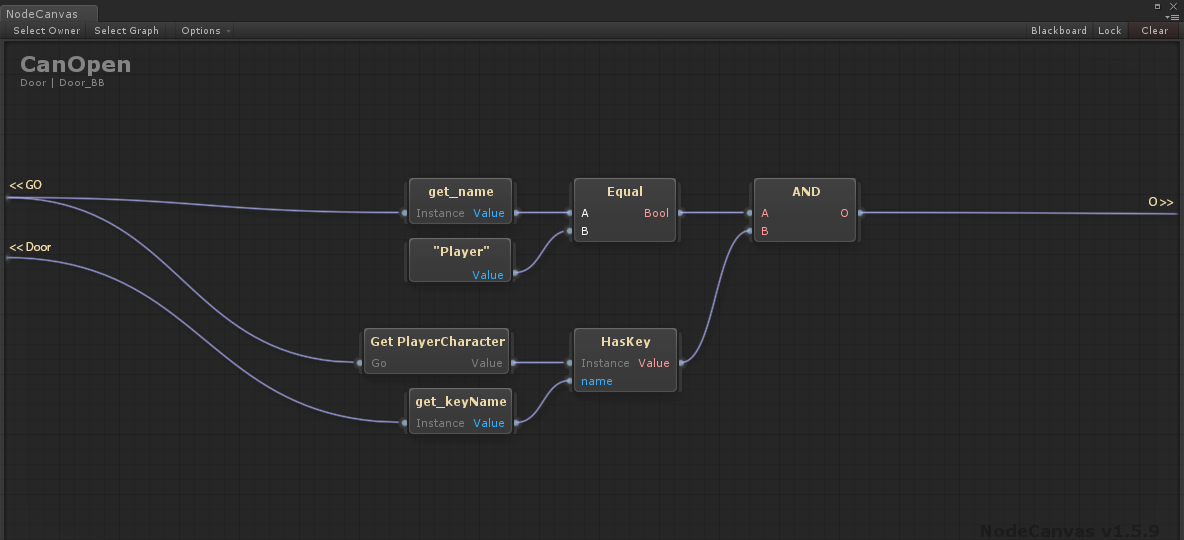
\includegraphics[width=\linewidth,height=\textheight,keepaspectratio]{VisualScriptingExample}
    \caption{Voorbeeld van een visuele script taal.}
\end{figure}

Daarnaast word de mogelijkheden van de visuele programmeer taal ook vaak gelimiteerd om het de gebruiker makkelijker te maken en het programma te beschermen van de gebruiker. Meestal als de limitaties van \gls{vs} een probleem worden had de logica beter in een tekstuele taal geschreven kunnen worden.

\section{Use Case's}
Door de jaren heen zijn er voor verschillende doeleinden visuele programmeer talen gemaakt. 
Een aantal voorbeelden zijn

\begin{itemize}  
\item Data flow in applicaties 
\item State flow voor onder andere animaties 
\item Geluids effecten programmeren
\item Gameplay Logica 
\item Programeren leren aan beginners 
\end{itemize}

In deze scriptie word er gefocust op het gebruik van \gls{vr} voor gameplay logica.

\section{Blueprints}
Blueprints is het visuele scripting systeem van \gls{ue4} en wat deze scriptie mogelijk maakt. De beschrijving van Unreal zelf is als volgt:

“Blueprints are special assets that provide an intuitive, node-based interface that can be used to create new types of Actors and script level events; giving designers and gameplay programmers the tools to quickly create and iterate gameplay from within Unreal Editor without ever needing to write a line of code.”

Blueprints ziet er als volgt uit:

\begin{figure}[H]
  \centering
    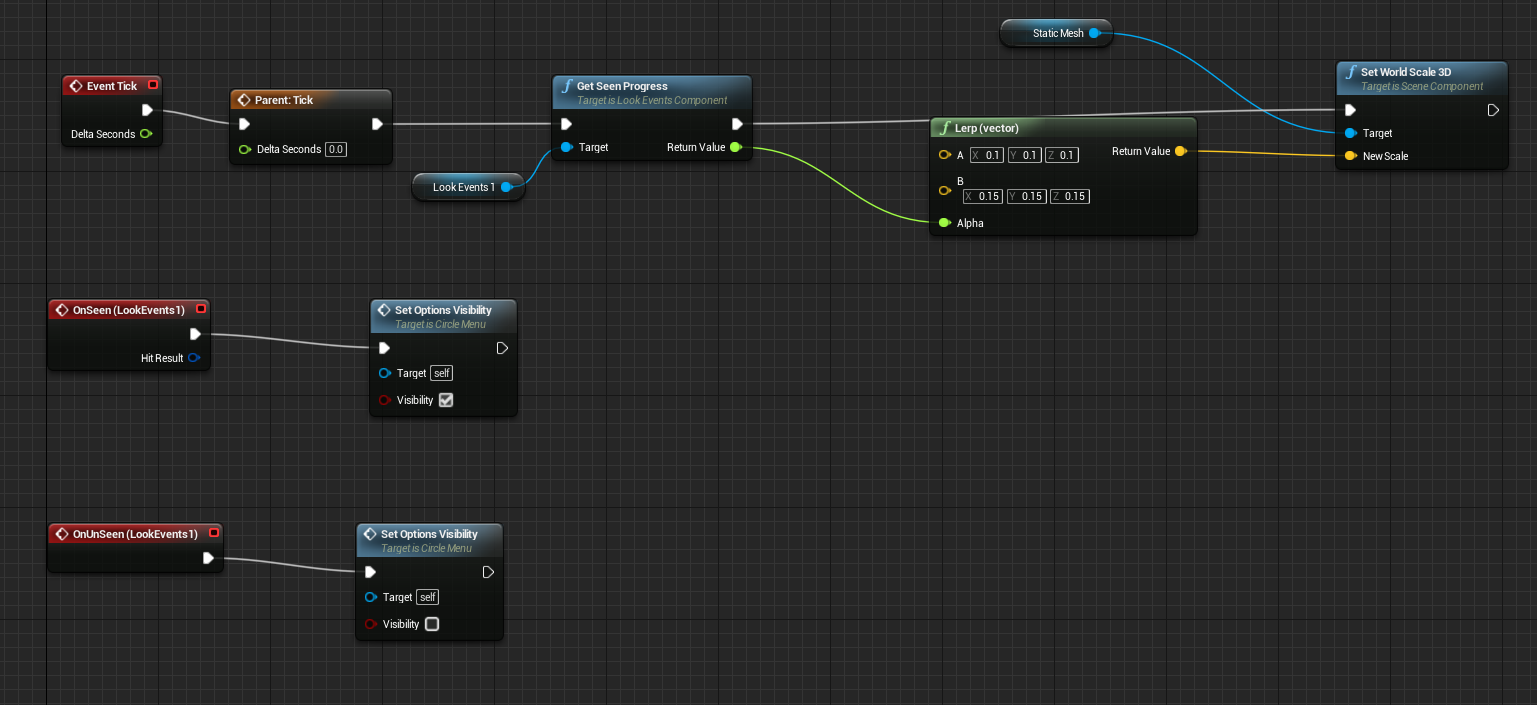
\includegraphics[width=\linewidth,height=\textheight,keepaspectratio]{BluePrintSeenExample}
    \caption{Voorbeeld van een Blueprint.}
\end{figure}

Een hele kort samenvatting zou zijn dat de rode nodes Events zijn en dus aangeven wanneer iets gebeurd, de witte lijnen bepalen de volgorde waarin de nodes worden uitgevoerd, de blauwe nodes zijn functies en de rest zijn variabelen of pure transformatie van data.

\section{Gameplay Logica}
Het programmeren van gameplay in een spel bestaat voor een groot gedeelte uit de vragen “Wanneer moet iets gebeuren”, “Wat moet er gebeuren” en “Hoe moet dit gebeuren”.
De vragen “Waarom moet iets gebeuren” en “Waar moet dit gebeuren” komen het meeste voor in de gameplay logica van een spel, vaak hebben deze vragen ook een makkelijk antwoord. Helaas zijn deze vragen lastig om te beantwoorden in tekstuele code.

\subsection{Het afvuren van een projectiel}
Een voorbeeld van deze drie vragen in code is als volgt, voor het voorbeeld laten wij de logica zien van het schieten van een projectiel in c++ gebaseerd op het standaard voorbeeld van een speler uit de \gls{ue4}.

\subsubsection{Tekstuele Implementatie}
In een c++ header bestand registreren wij de volgende functie in onze speler classe.
\begin{lstlisting}[caption=Registratie van de OnFire functie]
void OnFire();
\end{lstlisting}
Dan tijdens het opzetten van de input voor ons karakter laten we weten wanneer we een projectiel willen schieten.

\begin{lstlisting}[caption=Koppellen van de Fire actie aan de OndFire functie]
if( EnableTouchscreenMovement(InputComponent) == false )
{
	InputComponent->BindAction(
		"Fire", 
		IE_Pressed, 
		this, 
		&Adpi_unreal_colosseumCharacter::OnFire
	);
}
\end{lstlisting}
Maar omdat de “fire” actie niet werkt op een touch interface moeten we de onfire zelf afvuren als iemand het scherm aanraakt (De logica achter het registeren van touch events word niet getoond maar is wel aanwezig in de speler klasse).

\begin{lstlisting}[caption=Aanroepen van de OnFire functie tijdens het EndTouch event]
void Adpi_unreal_colosseumCharacter::EndTouch(const ETouchIndex::Type FingerIndex, const FVector Location)
{
	if (TouchItem.bIsPressed == false)
	{
		return;
	}
	if( ( FingerIndex == TouchItem.FingerIndex ) && (TouchItem.bMoved == false) )
	{
		OnFire();
	}
	TouchItem.bIsPressed = false;
}
\end{lstlisting}
Vervolgens definiëren we OnFire als volgt

\begin{lstlisting}[caption=Implementatie van de OnFire functie]
void Adpi_unreal_colosseumCharacter::OnFire()
{ 
	// try and fire a projectile
	if (ProjectileClass != NULL)
	{
		const FRotator SpawnRotation = GetControlRotation();
		// MuzzleOffset is in camera space, so transform it to world space before offsetting from the character location to find the final muzzle position
		const FVector SpawnLocation = GetActorLocation() + SpawnRotation.RotateVector(GunOffset);

		UWorld* const World = GetWorld();
		if (World != NULL)
		{
			// spawn the projectile at the muzzle
			World->SpawnActor<Adpi_unreal_colosseumProjectile>(ProjectileClass, SpawnLocation, SpawnRotation);
		}
	}

	// try and play the sound and fire animtation if specified
	...

}
\end{lstlisting}
Om de logica te implementeren voor het vuren vuren van de kogel hebben wij nu op vier verschillende plekken de logica moeten verspreiden, hiervan zit de implementatie verspreid in een bestand van 218 regels \ref{appendix:dpi_unreal_colosseumCharacter}.

\subsubsection{Visuele Implementatie}
De “Hoe moet dit gebeuren” is een complexe vraag die prima beantwoord word in code. Vooral omdat er verschillende logica achter elkaar plaatsvind, geluid afspelen / animatie starten, en een aantal wiskundige berekeningen. 

Maar de “Wanneer” vraag is makkelijk te beantwoorden. Namelijk als de fire actie uitgevoerd word of als er op het scherm gedrukt word. De logica in blueprints ziet er als volgt uit (in de event graph van een playerCharacter).

\begin{figure}[!ht]
  \centering
    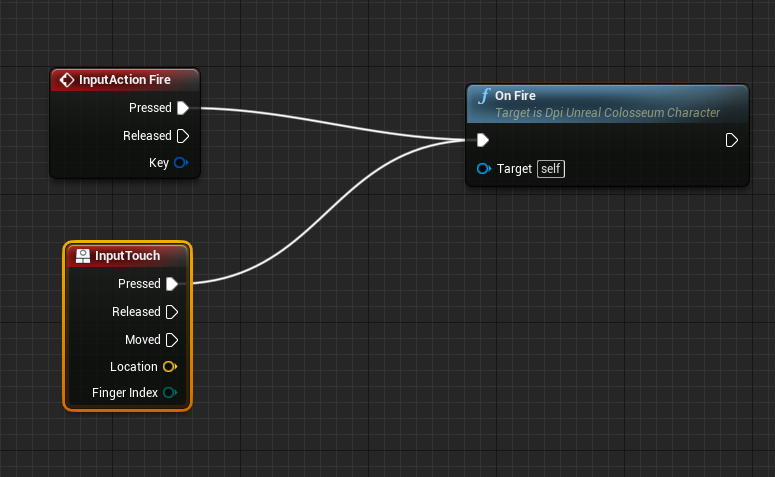
\includegraphics[width=\linewidth,height=\textheight,keepaspectratio]{OnFireBlueprintCall}
    \caption{Afvuren van een projectiel in Blueprints.}
\end{figure}

In tegenstelling tot de c++ code is de logica van de “Wanneer” vraag dit maal niet verspreid en is het in een oog opslag duidelijk wat er voor zorgt dat er een projectiel geschoten word. 

%!TEX root = ../Thesis.tex
\chapter{Unreal Engine 4}
In dit hoofdstuk word de keuze voor \gls{ue4} uitgelegd en een vergelijking gemaakt met andere engine's.
Ook word een korte introductie gemaakt voor Blueprints.

\section{Waarom de Unreal Engine 4}

Tijdens het kiezen van een Engine waren er drie rand voorwaarden namelijk 
\begin{enumerate}
	\item gratis voor educatie, of goedkoop genoeg voor DPI om aan te schaffen
	\item Oculus en GearVR ondersteuning
	\item Een \gls{vr} systeem
\end{enumerate}

De volgende Engine’s zijn naar gekeken 
\begin{itemize}
\item Unity
\item CRYENGINE
\item Unreal Engine 4
\end{itemize}

\subsection{Unity}

\subsubsection{Licentie}
Unity heeft een educatie licentie waaronder het grootste gedeelte van de engine gratis gebruikt kan worden maar rekening houdend met de interesses van DPI, en eventuele vervolg projecten die zei willen ondernemen, zal de licentie minimaal 75€ per maand worden met daar de koste van Android builds bij.

\subsubsection{Oculus en GearVR ondersteuning}
Van de drie engine’s heeft unity de meest uitgebreide platform support. Daarnaast is Unity vaak een van de eerste keuze’s om nieuwe technieken mee te implementeren. De reden achter deze keuze is het gemak waarop plugins gemaakt kunnen worden en de voordelige / gratis pricing van Unity wat het een populaire keuze maakt voor experimenteren.

\subsubsection{Virtual Scripting}
Unity heeft zelf niet een ingebouwd \gls{vs} systeem maar via een aantal plugins kan dit wel worden toegevoegd. Deze plugins zitten wel vast aan de limitaties van een Unity Plugin. Daarnaast word dit niet officieel gesupporterd door Untiy zelf.

\subsubsection{Gebruiks gemak}
Op gebruiksgemak, in serieuze projecten, fidelity en performance loopt Unity ver achter op de \gls{ue4} en CryEngine. Onderhoudbaar en uitbreidbaarheid van Unity is meestal rampzalig door de manier waarop code voor Unity geschreven word. Vaak is Unity daarom ook niet de keuze voor grote games van hoge kwaliteit. 

Het programmeren word namelijk in een component style in c-sharp gedaan. Het programmeren in c-sharp is voor veel mensen fijn omdat dit vaak een bekende taal is. Maar het component systeem en de manier waarop Unity relatie’s afhandelt zorgt dat er extreem snel spaghetti code ontstaat. 

\subsection{CRYENGINE}
\subsubsection{Licentie}
De CRYENGINE licentie bestaat uit een “Pay what you want” model. Daarnaast beid Crytek een “CRYENGINE Insider Membership“ aan voor 50€ of 150€. 

\subsubsection{Oculus en GearVR ondersteuning}
Op het moment van schrijven ondersteund de CRYENGINE wel de Oculus maar niet de GearVR. Android ondersteuning is mogelijk maar niet officieel ondersteund door Crytek. Dit zal het lastig maken om GearVR te ondersteunen.

\subsubsection{Visual Scripting}
De CRYENGINE heeft een ingebouwd \gls{vs} systeem genaamd Flow. Dit systeem heeft helaas geen ondersteuning voor overerving en de koppeling met c++ bestaat alleen uit het maken van nieuwe nodes en het aanspreken van graphs in c++.

\subsubsection{Gebruiksgemak}
De CryEngine staat bekend als een moeilijke Engine om in te beginnen maar heeft ondertussen bewezen een goede keuze te zijn voor game ontwikkelaars en grotere teams.

Door het gebrek aan persoonlijke ervaring kan ik hier minder over zeggen. Maar door het gebrek aan GearVR ondersteuning is er hier niet meer in verdiept.

\subsection{Unreal Engine 4}
\subsubsection{Licentie}
Het gebruik van de \gls{ue4} is compleet gratis voor educatie en niet-game applicaties zoals architectuur, visualisatie, films etc. Dit betekend dat zowel tijdens het afstuderen als mogelijke vervolg projecten van DPI er geen licentie kosten betaald hoeven te worden.

\subsubsection{Oculus en GearVR ondersteuning}
\gls{ue4} ondersteund zowel de Oculus als Gear VR. Daarnaast ondersteund het ook de meeste randapparatuur voor \gls{vr} zoals Leap Motion en Kinect. Updates hiervoor komen vaak wel later dan voor Unity.
\subsubsection{Visual Scripting}
Unreal heeft een uitgebreid \gls{vs} systeem wat nauw samenwerkt met c++. Alle functies die in c++ beschikbaar zijn zijn beschikbaar via Blueprints. Van elke Blueprint kan ook direct de source code ingesprongen worden, zelfs voor de functies uit de \gls{ue4} libraries.

Het koppelen van c++ aan Blueprints is vrij simpel en ondersteund ook het creëren van events in c++ en functionaliteit hieraan via Blueprints te koppelen.

\subsubsection{Gebruiks gemak}
De leer curve van \gls{ue4} is redelijk stijl maar binnen een paar weken is het mogelijk de belangrijkste te leren. Een punt om rekening mee te houden is dat het zomaar iets maken in de \gls{ue4} vaak verkeerd uitpakt. Daarom is het belangrijk de documentatie, van het onderdeel waar je mee bezig bent, goed te lezen.

Als de basis principes eenmaal onder de knie zijn kan er extreem snel ontwikkeld, en geprototyped, worden met de \gls{ue4} door de implementatie van \gls{vs} en een strakke en goed uitgedachte UI.

\subsubsection{Conclusie}
De CRYENGINE valt af vanwege zijn gebrek aan GearVR support. Dan blijft de keuze over tussen Unity en \gls{ue4}. Untiy heeft een minder style learning curve maar geavanceerde 3D technieken zullen uiteindelijk toch geleerd moeten worden om een hoge kwaliteit te behalen. 

Het visuele scripting systeem van Unity is beperkt en mist de kracht en flexibiliteit die nodig is om deze scriptie succesvol af te ronden. Daar in tegen beid het visuele scripting systeem van \gls{ue4} wel deze mogelijkheden.

\section{Blueprints}
Blueprints is het visuele scripting systeem van \gls{ue4} en wat deze scriptie mogelijk maakt. De beschrijving van Unreal zelf is als volgt:

“Blueprints are special assets that provide an intuitive, node-based interface that can be used to create new types of Actors and script level events; giving designers and gameplay programmers the tools to quickly create and iterate gameplay from within Unreal Editor without ever needing to write a line of code.”

Blueprints ziet er als volgt uit:

\begin{figure}[!ht]
  \centering
    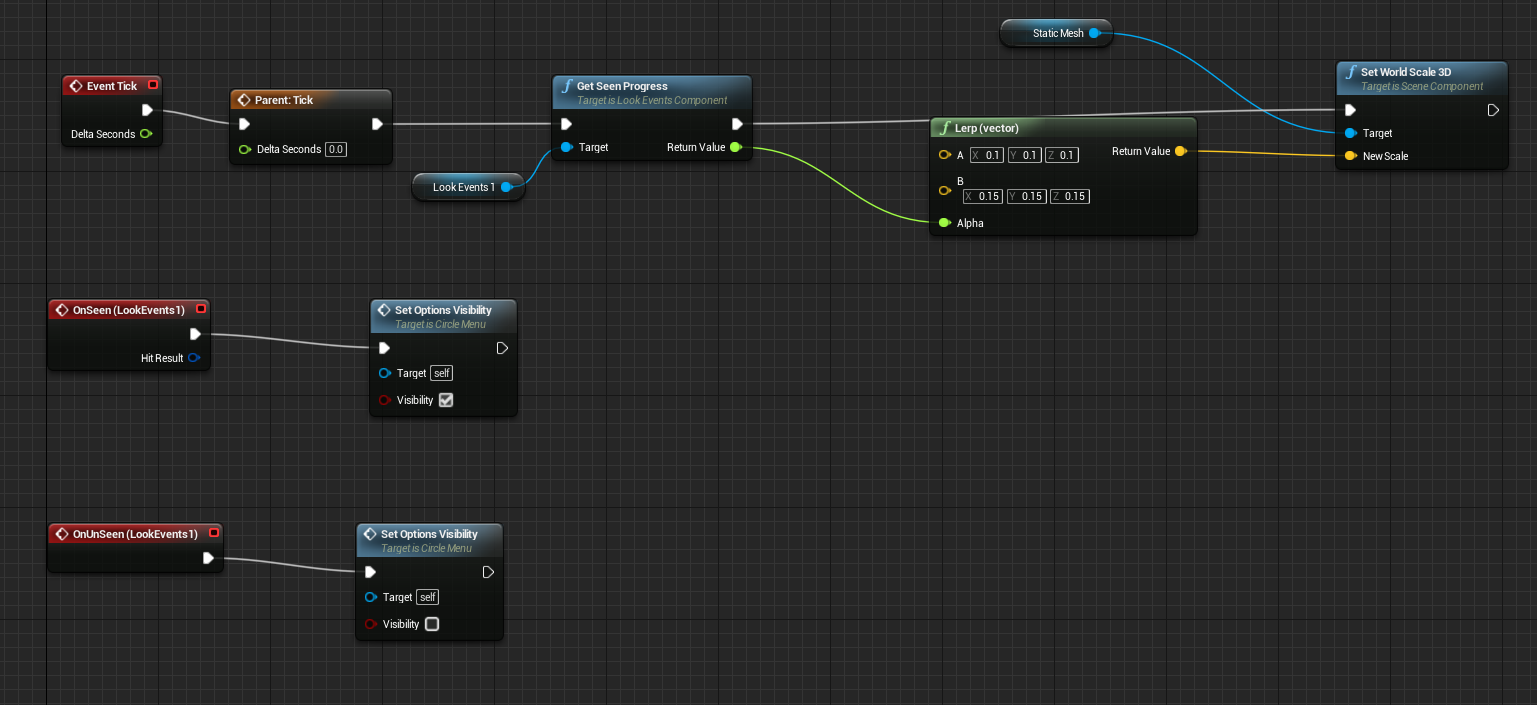
\includegraphics[width=\linewidth,height=\textheight,keepaspectratio]{BluePrintSeenExample}
    \caption{Voorbeeld van een Blueprint.}
\end{figure}

Een hele kort samenvatting zou zijn dat de rode nodes Events zijn en dus aangeven wanneer iets gebeurd, de witte lijnen bepalen de volgorde waarin de nodes worden uitgevoerd, de blauwe nodes zijn functies en de rest zijn variabelen of pure transformatie van data. 

%!TEX root = ../Thesis.tex
\lstset {language=C++}
% Define block styles
\tikzstyle{decision} = [diamond, draw, fill=blue!20, 
    text width=4.5em, text badly centered, node distance=3cm, inner sep=0pt]
\tikzstyle{block} = [rectangle, draw, fill=blue!20, 
    text width=5em, text centered, rounded corners, minimum height=4em]
\tikzstyle{line} = [draw, -latex']
\tikzstyle{cloud} = [draw, ellipse,fill=red!20, node distance=3cm,
    minimum height=2em]

\chapter{Blueprints en C++}

In dit hoofdstuk word gameplay logica in drie aspecten verdeeld en word voor elk aspect naar de voor en nadelen van C++ en Blueprints gekeken.

Aan de hand van deze vergelijkingen word een workflow gekozen voor het programmeren van deze logica waarin wij het beste uit C++ en Blueprints proberen te combineren.

\section{Gameplay}

Om de scheiding tussen c++ en Blueprints concreet te maken verdelen wij gameplay logica in de volgende vragen:

\begin{itemize}
	\item Wanneer moet iets gebeuren
	\item Wat moet er gebeuren
	\item Hoe moet dit gebeuren
\end{itemize}

Door deze scheiding wordt het makkelijker om de keuze tussen een C++ en een Blueprint implementatie te maken en kunnen er een aantal richtlijnen opgezet worden.

\subsection{Wanneer}
De wanneer vragen zijn vaak makkelijk te beantwoorden, bijvoorbeeld als de speler geraakt word door een projectiel wil ik dat geluid x afgespeeld word, maar moeilijk te coderen door hun asynchrone natuur. Een van de krachtigste voordelen van een Visuele programmeer taal is dat de flow van een programma uitgedrukt kan worden door middel van de lijnen tussen nodes. 

Om het verschil tussen asynchrone logica in C++ en blueprints duidelijk te maken implementeren wij hieronder het afspelen van een geluid nadat een speler dood gaat.

\subsubsection{C++}
We registeren eerst een functie die aangesproken kan worden door de timeout en het geluid wat afgespeeld word in de header van de character.

\begin{lstlisting}	
/** Plays a sound x seconds after the death of the player*/
void AfterDeathSoundTimeOut();

/** Sound to play each time we fire */
UPROPERTY(EditAnywhere, BlueprintReadWrite, Category=Gameplay)
class USoundBase* DeathSound;
\end{lstlisting}

Vervolgens word deze functie geïmplementeerd in de character.cpp

\begin{lstlisting}
void Adpi_unreal_colosseumCharacter::AfterDeathSoundTimeOut() 
{
	UGameplayStatics::PlaySoundAtLocation(this, FireSound, GetActorLocation());
}
\end{lstlisting}

En word de timeout voor het geluid gezet tijdens het doodgaan van de speler.

\begin{lstlisting}
void Adpi_unreal_colosseumCharacter::OnDeath(const FDeathReason Reason)
{
	// death logic
	...

	FTimerHandle UnusedHandler= FTimerHandle();
	GetWorld()->GetTimerManager().SetTimer(
		UnusedHandler, 
		this, 
		&Adpi_unreal_colosseumCharacter::AfterDeathSoundTimeOut, 
		1.0f
	);
}
\end{lstlisting}

We zien hier dat de gerelateerde code op drie verschillende plekken komt te staan, tussen niet relevante code in. Pas na het lezen van de code op deze drie plekken word het duidelijk wat de complete functionaliteit is. Er zijn hier natuurlijk hulpmiddel voor zoals opmerkingen boven code te plaatsen maar bij elke extra taak die, asynchroon, uitgevoerd moet worden word de code complexer en moeilijker te begrijpen. De lezer moet namelijk alle gerelateerde functionaliteit in zijn geheugen hebben.

\subsubsection{Blueprints}
In Blueprints zou deze logica er als volgt uit zien:

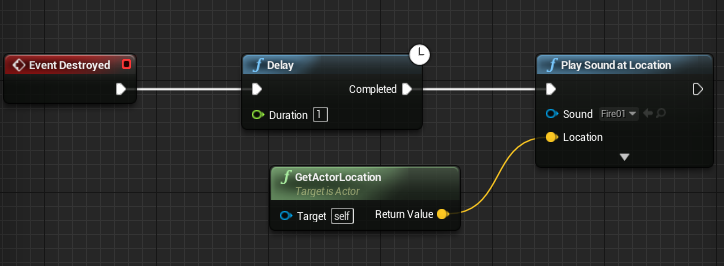
\includegraphics{OnDestroyedSoundDelay}

In de blueprint implementatie is het in een oog opslag duidelijk dat er een geluid afgespeeld word op de locatie van de speler een seconde nadat deze deze dood gaat. De logica bevind zich op de dezelfde plek en de witte lijnen geven de flow van de logica aan. 

Een ander groot verschil dat we hier zien is dat er voor iets simpels als een vertraging in tekstuele code naast de standaard kennis van de c++ syntax ook kennis nodig is van de volgende concepten:

\begin{itemize}
	\item Pointers
	\item Pass by reference
	\item Function references
	\item Namespaces
	\item Out parameters (de UnusedHandler)
	\item Floats
	\item Types
	\item Macros. 
\end{itemize}

Terwijl in Blueprints all deze concepten verborgen zijn in de nodes. Het verbergen van de onderliggende werking van functionaliteit is een thema wat vaker terugkomt in programmeren en wordt aangemoedigd. Het verbergen van deze logica heeft als gevolg dat er zonder programmeer kennis de wanneer logica geïmplementeerd kan worden.

\subsection{Wat}

Het plaatsen van de wat logica in Blueprints of c++ is lastiger om te bepalen. Voor logica die de niet-programmeurs schrijven is c++ geen optie en moet dit wel in Blueprints maar voor programmeurs moet er een afweging gemaakt worden.

Het probleem ontstaat voornamelijk bij complexe conditionele logica.

\subsubsection{Conditionele Logica}

Als we de conditionele logica van het afvuren van de events van een.
LookEventsComponent[zie hoofstuk ?] in c++ en blueprints met elkaar vergelijken.

\begin{itemize}
	\item Bijlage 1: Tick functie van de LookEventsComponent \ref{appendix:LookEventsLogicC}
	\item Bijlage 2: Conditional logic van Tick functie van LookEvents in Blueprints \ref{appendix:LookEventsLogicBlueprints}
\end{itemize}

Zijn beide varianten moeilijk te lezen. Voor iemand die niet codeert ziet de Blueprints variant er waarschijnlijk begrijpgaarder uit maar de complexiteit komt voornamelijk door de logica zelf en in tekstuele code zijn er een aantal manieren om dit soort constructies kleiner te maken zoals:

\begin{lstlisting}
if (bActive != true || (bShouldUsedOnce && TimesUsed > 0) || bIsInTimeOut == true) 
{
	return;
}
\end{lstlisting}
In vergelijking met 

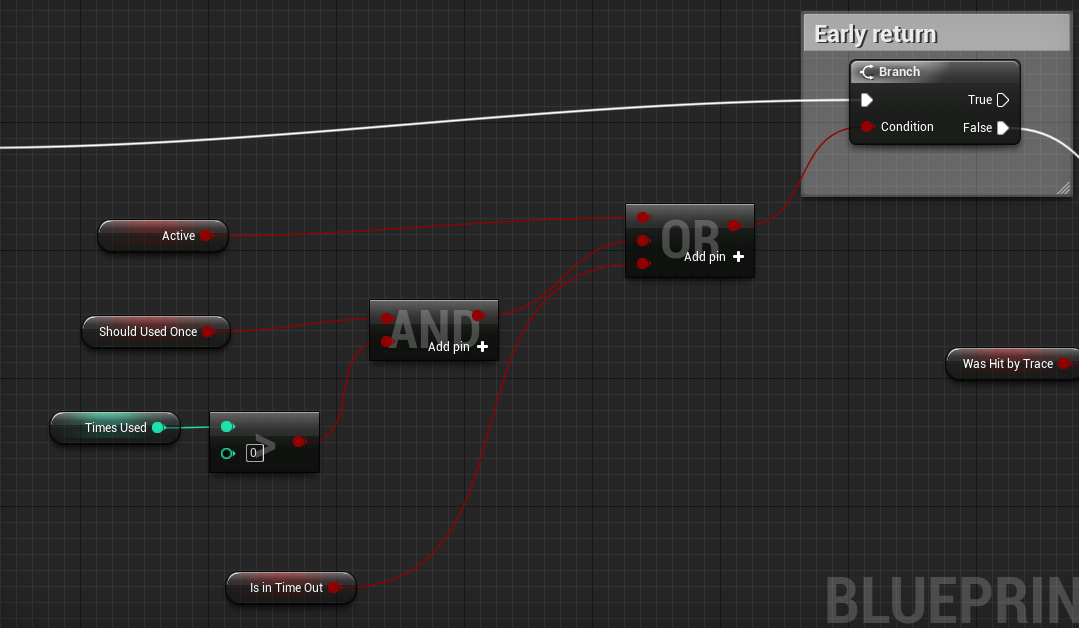
\includegraphics{EarlyReturnBluePrint}

Een ander voorbeeld is de volgende functie die bepaald of de trigger van een LookEventsComponent onderdeel was van een trace.

\begin{lstlisting}
FHitResult ULookEventsComponent::WasHitByTrace(const TArray<FHitResult> HitResults) 
{
	UObject* Trigger = (bIsBeingWatched) ? UnSeenTrigger : SeenTrigger;

	for (auto& HitResult : HitResults)
	{
		UObject* HitObject = (Trigger->IsA(AActor::StaticClass())) ? Cast<UObject>(HitResult.GetActor()) : Cast<UObject>(HitResult.GetComponent());	

		if (HitObject == Trigger)
		{
			if (bShouldDrawTriggerDebug) {
				DebugTrigger(HitObject, 0.1f);
			}
			return HitResult;
		}
	}
	return FHitResult();
}
\end{lstlisting}

In vergelijking met:

\includegraphics{WasHitBytTraceBluePrintExample}

Voor complexe conditionele logica is c++ sneller te begrijpen en geeft meer mogelijkheden om dit te versimpelen. 

\subsection{Hoe}
Met de hoe vraag word de interne werking van een functionaliteit bedoelt waaronder ook de integratie met de rest van het programma, denk aan integratie met de rest van de engine, lifecycles, overerving en performance.

Complexe algoritmes zijn altijd makkelijker in C++ voor zowel leesbaarheid als onderhoudbaarheid. Daarnaast is de scheiding van algoritmes met de rest van de code belangrijk voor het scheiden van complexiteit.

\subsection{Onderhoud en Performance}
Naast het schrijven van de logica zijn performance en onderhoud twee onderwerpen die door elk aspect van een spel verwikkeld zijn en daarom ook onderdeel moeten zijn voor onze keuze van workflow.

\subsubsection{Onderhoud}
Naast een kleine verbetering in leesbaarheid heeft het schrijven van logica in c++ een ander belangrijke voordelen. Namelijk de voordelen van een code editor. Dit geeft uitgebreide debug, zoek en meta informatie. 

De error’s die de Unreal Engine 4 voor je genereed zijn niet altijd even duidelijk, voornamelijk error’s die pas tijdens het packagen van een project ontstaan, en het vinden van een foutieve Blueprint kan extreem lastig zijn. Bijna elk element in de Unreal Engine 4 kan Blueprints code bevatten. En elk element op zich kan die Blueprints weer in kleinere elementen verdelen. Deze elementen bevinden zich tussen alle andere soorten assets zoals Meshes, Animaties, Deciscion Trees, Materials, Textures etc en het zoeken van een onbekende fout hierin is extreem lastig.

Als de foutieve code in c++ had gestaan kan er altijd door middel van een stack trace gekeken worden in welke functie het fout gaat en kan er gezien worden welke functie die functie aansprak en verder omhoog. 

Het auto aan vullen van functie namen en informatie tonen over functies door middel van de JavaDoc opmerking notatie versimpelt het schrijven van complexe code die gebruikt maakt van de Unreal Engine 4. 

\subsubsection{Performance}
Een ander belangrijk onderdeel van de hoe logica is performance. De performance van Blueprints is namelijk lager dan dat van c++. In de hoe en wat vraag is dit verschil compleet onmerkbaar maar in code wat vaak, bijvoorbeeld in de loop van een game, word uitgevoerd kan het verschil merkbaar worden.
In c++ is er ook veel meer controle over de manier waarop de computer logica interpreteert, in Blueprints is dit een stuk minder duidelijk. Dit zorgt ervoor dat op een lager niveau optimalisaties mogelijk zijn. 

Daarnaast is het makkelijker om complexe optimalisaties te schrijven op een onderhoudbaar manier. Als er bijvoorbeeld een performance probleem ontstaat in het aantal raytraces wat de LookEventsComponents nodig hebben is het mogelijk om een cache te schrijven voor de ray traces waar de LookEventsComponent een trace uit vraagt als deze trace dan al eerder door een andere LookEventsComponent berekend is krijg hij de resultaten van die trace inplaats van een nieuwe trace te maken.

\subsection{Conclusie}
Voor de wanneer vraag is Blueprints voor zowel de programmeur als de niet-programmeur altijd de beste optie. Niet alleen is het leesbaarder maar ook flexibeler doordat de logica op een logische manier achter elkaar staat.

Voor de hoe vraag is C++ altijd de beste optie. Onderhoudbaarheid en performance spelen hier een belangrijke rol. 

Voor de wat vraag heeft de niet-programmeur geen optie maar de programmeur wel. Voor triviale code kan er gekozen worden voor Blueprints maar voor complexe conditionele logica heeft C++ de voorkeur. 

\section{Workflow}
Voor onze workflow willen wij de complexiteit voor de niet-programmeurs zo laag mogelijk houden met zo veel mogelijk vrijheid. Daarnaast is flexibiliteit belangrijk voor het makkelijk en veilig experimenteren en itereren.

Gebaseerd op het verdelen van de gameplay logica in de drie vragen hoe, wat en wanneer word er voor de volgende workflow gekozen.
    
\begin{center}
	\begin{tikzpicture}
		[node distance=.8cm,
		start chain=going below,]
			\node[punktchain, join] (Experimenteren) 	
				{Experimenteren (Blueprints)};
			\node[punktchain, join] (hoe)      			
				{Implementatie hoe (C++)};
			\node[punktchain, join] (wat)    			
				{Implementatie complexe wat (C++)};
			\node[punktchain, join] (overerving) 		
				{Blueprints overerving (Blueprints)};
			\node[punktchain, join] (wanneer) 			
				{Wanner en wat (Blueprints)};
	\end{tikzpicture}
\end{center}

Elk component zal beginnen als een imperfecte Blueprint logica. In dit stadium is de performance en onderhoud niet belangrijk, en hoeft het niet eens compleet functioneel te zijn. Er kan direct ge-experimenteert en getest worden. Dit kan niet alleen waardevolle informatie opleveren voor het design aspect van een project maar plaats de logica ook in de context van het project. Vaak komt hier gewenste functionaliteit uit die tijdens het bedenken over het hoofd gekeken is.

Nadat het duidelijk is dat het component gebruikt gaat worden in het project en de gewenste functionaliteiten duidelijk zijn kan er een fatsoenlijke en efficiënte C++ implementatie geschreven worden.

De C++ implementatie word vervolgens overerft door een Blueprint die de aanvullende logica toevoegt.

Ook in gevallen waarin de Blueprint niet iets toe te voegen heeft is het belangrijk om toch een Blueprint te maken van de C++ code. Er kan hierdoor namelijk makkelijk mee geëxperimenteerd worden en niet-programmeurs hebben hierdoor ook de mogelijkheid om iets toe te voegen of een standaard waarde te veranderen.

\section{Versie Controle}
Versie controle is een belangrijk onderdeel van elk ICT project en al valt dit buiten de scope van deze scriptie word er hier een korte vermelding van gemaakt.

Versie controle is een belangrijk onderdeel in samen werken aan code en speelt een belangrijke rol in het onderhoud van code. Er zijn tools in Unreal Engine 4 om versie controle tools zoals git en svn op Blueprints, en assets, toe te passen. Voor deze scriptie is de plugin ontwikkeld met behulp van git maar is er niet gekeken naar een manier waarop niet-programmeurs hier ook mee kunnen werken.

Tijdens de interviews[?] werd het duidelijk dat er geen bestaande kennis van versie controle aanwezig was in de visuele teams van DPI. Het kiezen, opzetten en leren van versie controle en de integratie hiervan met de Unreal Engine 4 valt buiten de scope van deze scriptie.

%\input{Chapters/Chapter5} % Experiment 2

%\input{Chapters/Chapter6} % Results and Discussion

%\input{Chapters/Chapter7} % Conclusion

%% ----------------------------------------------------------------
% Now begin the Appendices, including them as separate files

\addtocontents{toc}{\vspace{2em}} % Add a gap in the Contents, for aesthetics

\appendix % Cue to tell LaTeX that the following 'chapters' are Appendices

%!TEX root = ../Thesis.tex
\lstset {language=C++}

\chapter{Implementatie voorbeeld speler Unreal Engine 4}
\label{appendix:dpi_unreal_colosseumCharacter}

\begin{lstlisting}[
	basicstyle=\tiny, 
	caption={dpi unreal colosseumCharacter header}, 
	label={dpiunrealcolosseumCharacterheader}
]
#pragma once
#include "GameFramework/Character.h"
#include "dpi_unreal_colosseumCharacter.generated.h"

class UInputComponent;

UCLASS(config=Game)
class Adpi_unreal_colosseumCharacter : public ACharacter
{
	GENERATED_BODY()

	/** Pawn mesh: 1st person view (arms; seen only by self) */
	UPROPERTY(VisibleDefaultsOnly, Category=Mesh)
	class USkeletalMeshComponent* Mesh1P;

	/** Gun mesh: 1st person view (seen only by self) */
	UPROPERTY(VisibleDefaultsOnly, Category = Mesh)
	class USkeletalMeshComponent* FP_Gun;

	/** First person camera */
	UPROPERTY(VisibleAnywhere, BlueprintReadOnly, Category = Camera, meta = (AllowPrivateAccess = "true"))
	class UCameraComponent* FirstPersonCameraComponent;
public:
	Adpi_unreal_colosseumCharacter();

	/** Base turn rate, in deg/sec. Other scaling may affect final turn rate. */
	UPROPERTY(VisibleAnywhere, BlueprintReadOnly, Category=Camera)
	float BaseTurnRate;

	/** Base look up/down rate, in deg/sec. Other scaling may affect final rate. */
	UPROPERTY(VisibleAnywhere, BlueprintReadOnly, Category=Camera)
	float BaseLookUpRate;

	/** Gun muzzle's offset from the characters location */
	UPROPERTY(EditAnywhere, BlueprintReadWrite, Category=Gameplay)
	FVector GunOffset;

	/** Projectile class to spawn */
	UPROPERTY(EditDefaultsOnly, Category=Projectile)
	TSubclassOf<class Adpi_unreal_colosseumProjectile> ProjectileClass;

	/** Sound to play each time we fire */
	UPROPERTY(EditAnywhere, BlueprintReadWrite, Category=Gameplay)
	class USoundBase* FireSound;

	/** AnimMontage to play each time we fire */
	UPROPERTY(EditAnywhere, BlueprintReadWrite, Category = Gameplay)
	class UAnimMontage* FireAnimation;

protected:
	
	/** Fires a projectile. */
	void OnFire();

	/** Handles moving forward/backward */
	void MoveForward(float Val);

	/** Handles stafing movement, left and right */
	void MoveRight(float Val);

	/**
	 * Called via input to turn at a given rate.
	 * @param Rate	This is a normalized rate, i.e. 1.0 means 100% of desired turn rate
	 */
	void TurnAtRate(float Rate);

	/**
	 * Called via input to turn look up/down at a given rate.
	 * @param Rate	This is a normalized rate, i.e. 1.0 means 100% of desired turn rate
	 */
	void LookUpAtRate(float Rate);

	struct TouchData
	{
		TouchData() { bIsPressed = false;Location=FVector::ZeroVector;}
		bool bIsPressed;
		ETouchIndex::Type FingerIndex;
		FVector Location;
		bool bMoved;
	};
	void BeginTouch(const ETouchIndex::Type FingerIndex, const FVector Location);
	void EndTouch(const ETouchIndex::Type FingerIndex, const FVector Location);
	void TouchUpdate(const ETouchIndex::Type FingerIndex, const FVector Location);
	TouchData	TouchItem;
	
protected:
	// APawn interface
	virtual void SetupPlayerInputComponent(UInputComponent* InputComponent) override;
	// End of APawn interface

	/* 
	 * Configures input for touchscreen devices if there is a valid touch interface for doing so 
	 *
	 * @param	InputComponent	The input component pointer to bind controls to
	 * @returns true if touch controls were enabled.
	 */
	bool EnableTouchscreenMovement(UInputComponent* InputComponent);

public:
	/** Returns Mesh1P subobject **/
	FORCEINLINE class USkeletalMeshComponent* GetMesh1P() const { return Mesh1P; }
	/** Returns FirstPersonCameraComponent subobject **/
	FORCEINLINE class UCameraComponent* GetFirstPersonCameraComponent() const { return FirstPersonCameraComponent; }

};

\end{lstlisting}

\begin{lstlisting}[
	basicstyle=\tiny, 
	caption={dpi unreal colosseumCharacter cpp}, 
	label={dpiunrealcolosseumCharactercpp}
]
#include "dpi_unreal_colosseum.h"
#include "dpi_unreal_colosseumCharacter.h"
#include "dpi_unreal_colosseumProjectile.h"
#include "Animation/AnimInstance.h"
#include "GameFramework/InputSettings.h"

DEFINE_LOG_CATEGORY_STATIC(LogFPChar, Warning, All);

//////////////////////////////////////////////////////////////////////////
// Adpi_unreal_colosseumCharacter

Adpi_unreal_colosseumCharacter::Adpi_unreal_colosseumCharacter()
{
	// Set size for collision capsule
	GetCapsuleComponent()->InitCapsuleSize(42.f, 96.0f);

	// set our turn rates for input
	BaseTurnRate = 45.f;
	BaseLookUpRate = 45.f;

	// Create a CameraComponent	
	FirstPersonCameraComponent = CreateDefaultSubobject<UCameraComponent>(TEXT("FirstPersonCamera"));
	FirstPersonCameraComponent->AttachParent = GetCapsuleComponent();
	FirstPersonCameraComponent->RelativeLocation = FVector(0, 0, 64.f); // Position the camera
	FirstPersonCameraComponent->bUsePawnControlRotation = true;

	// Create a mesh component that will be used when being viewed from a '1st person' view (when controlling this pawn)
	Mesh1P = CreateDefaultSubobject<USkeletalMeshComponent>(TEXT("CharacterMesh1P"));
	Mesh1P->SetOnlyOwnerSee(true);
	Mesh1P->AttachParent = FirstPersonCameraComponent;
	Mesh1P->bCastDynamicShadow = false;
	Mesh1P->CastShadow = false;

	// Create a gun mesh component
	FP_Gun = CreateDefaultSubobject<USkeletalMeshComponent>(TEXT("FP_Gun"));
	FP_Gun->SetOnlyOwnerSee(true);			// only the owning player will see this mesh
	FP_Gun->bCastDynamicShadow = false;
	FP_Gun->CastShadow = false;
	FP_Gun->AttachTo(Mesh1P, TEXT("GripPoint"), EAttachLocation::SnapToTargetIncludingScale, true);


	// Default offset from the character location for projectiles to spawn
	GunOffset = FVector(100.0f, 30.0f, 10.0f);

	// Note: The ProjectileClass and the skeletal mesh/anim blueprints for Mesh1P are set in the
	// derived blueprint asset named MyCharacter (to avoid direct content references in C++)
}

//////////////////////////////////////////////////////////////////////////
// Input

void Adpi_unreal_colosseumCharacter::SetupPlayerInputComponent(class UInputComponent* InputComponent)
{
	// set up gameplay key bindings
	check(InputComponent);

	InputComponent->BindAction("Jump", IE_Pressed, this, &ACharacter::Jump);
	InputComponent->BindAction("Jump", IE_Released, this, &ACharacter::StopJumping);
	
	//InputComponent->BindTouch(EInputEvent::IE_Pressed, this, &Adpi_unreal_colosseumCharacter::TouchStarted);
	if( EnableTouchscreenMovement(InputComponent) == false )
	{
		InputComponent->BindAction("Fire", IE_Pressed, this, &Adpi_unreal_colosseumCharacter::OnFire);
	}
	
	InputComponent->BindAxis("MoveForward", this, &Adpi_unreal_colosseumCharacter::MoveForward);
	InputComponent->BindAxis("MoveRight", this, &Adpi_unreal_colosseumCharacter::MoveRight);
	
	// We have 2 versions of the rotation bindings to handle different kinds of devices differently
	// "turn" handles devices that provide an absolute delta, such as a mouse.
	// "turnrate" is for devices that we choose to treat as a rate of change, such as an analog joystick
	InputComponent->BindAxis("Turn", this, &APawn::AddControllerYawInput);
	InputComponent->BindAxis("TurnRate", this, &Adpi_unreal_colosseumCharacter::TurnAtRate);
	InputComponent->BindAxis("LookUp", this, &APawn::AddControllerPitchInput);
	InputComponent->BindAxis("LookUpRate", this, &Adpi_unreal_colosseumCharacter::LookUpAtRate);
}

void Adpi_unreal_colosseumCharacter::OnFire()
{ 
	// try and fire a projectile
	if (ProjectileClass != NULL)
	{
		const FRotator SpawnRotation = GetControlRotation();
		// MuzzleOffset is in camera space, so transform it to world space before offsetting from the character location to find the final muzzle position
		const FVector SpawnLocation = GetActorLocation() + SpawnRotation.RotateVector(GunOffset);

		UWorld* const World = GetWorld();
		if (World != NULL)
		{
			// spawn the projectile at the muzzle
			World->SpawnActor<Adpi_unreal_colosseumProjectile>(ProjectileClass, SpawnLocation, SpawnRotation);
		}
	}

	// try and play the sound if specified
	if (FireSound != NULL)
	{
		UGameplayStatics::PlaySoundAtLocation(this, FireSound, GetActorLocation());
	}

	// try and play a firing animation if specified
	if(FireAnimation != NULL)
	{
		// Get the animation object for the arms mesh
		UAnimInstance* AnimInstance = Mesh1P->GetAnimInstance();
		if(AnimInstance != NULL)
		{
			AnimInstance->Montage_Play(FireAnimation, 1.f);
		}
	}

}

void Adpi_unreal_colosseumCharacter::BeginTouch(const ETouchIndex::Type FingerIndex, const FVector Location)
{
	if( TouchItem.bIsPressed == true )
	{
		return;
	}
	TouchItem.bIsPressed = true;
	TouchItem.FingerIndex = FingerIndex;
	TouchItem.Location = Location;
	TouchItem.bMoved = false;
}

void Adpi_unreal_colosseumCharacter::EndTouch(const ETouchIndex::Type FingerIndex, const FVector Location)
{
	if (TouchItem.bIsPressed == false)
	{
		return;
	}
	if( ( FingerIndex == TouchItem.FingerIndex ) && (TouchItem.bMoved == false) )
	{
		OnFire();
	}
	TouchItem.bIsPressed = false;
}

void Adpi_unreal_colosseumCharacter::TouchUpdate(const ETouchIndex::Type FingerIndex, const FVector Location)
{
	if ((TouchItem.bIsPressed == true) && ( TouchItem.FingerIndex==FingerIndex))
	{
		if (TouchItem.bIsPressed)
		{
			if (GetWorld() != nullptr)
			{
				UGameViewportClient* ViewportClient = GetWorld()->GetGameViewport();
				if (ViewportClient != nullptr)
				{
					FVector MoveDelta = Location - TouchItem.Location;
					FVector2D ScreenSize;
					ViewportClient->GetViewportSize(ScreenSize);
					FVector2D ScaledDelta = FVector2D( MoveDelta.X, MoveDelta.Y) / ScreenSize;									
					if (ScaledDelta.X != 0.0f)
					{
						TouchItem.bMoved = true;
						float Value = ScaledDelta.X * BaseTurnRate;
						AddControllerYawInput(Value);
					}
					if (ScaledDelta.Y != 0.0f)
					{
						TouchItem.bMoved = true;
						float Value = ScaledDelta.Y* BaseTurnRate;
						AddControllerPitchInput(Value);
					}
					TouchItem.Location = Location;
				}
				TouchItem.Location = Location;
			}
		}
	}
}

void Adpi_unreal_colosseumCharacter::MoveForward(float Value)
{
	if (Value != 0.0f)
	{
		// add movement in that direction
		AddMovementInput(GetActorForwardVector(), Value);
	}
}

void Adpi_unreal_colosseumCharacter::MoveRight(float Value)
{
	if (Value != 0.0f)
	{
		// add movement in that direction
		AddMovementInput(GetActorRightVector(), Value);
	}
}

void Adpi_unreal_colosseumCharacter::TurnAtRate(float Rate)
{
	// calculate delta for this frame from the rate information
	AddControllerYawInput(Rate * BaseTurnRate * GetWorld()->GetDeltaSeconds());
}

void Adpi_unreal_colosseumCharacter::LookUpAtRate(float Rate)
{
	// calculate delta for this frame from the rate information
	AddControllerPitchInput(Rate * BaseLookUpRate * GetWorld()->GetDeltaSeconds());
}

bool Adpi_unreal_colosseumCharacter::EnableTouchscreenMovement(class UInputComponent* InputComponent)
{
	bool bResult = false;
	if(FPlatformMisc::GetUseVirtualJoysticks() || GetDefault<UInputSettings>()->bUseMouseForTouch )
	{
		bResult = true;
		InputComponent->BindTouch(EInputEvent::IE_Pressed, this, &Adpi_unreal_colosseumCharacter::BeginTouch);
		InputComponent->BindTouch(EInputEvent::IE_Released, this, &Adpi_unreal_colosseumCharacter::EndTouch);
		InputComponent->BindTouch(EInputEvent::IE_Repeat, this, &Adpi_unreal_colosseumCharacter::TouchUpdate);
	}
	return bResult;
}

\end{lstlisting}
%!TEX root = ../Thesis.tex
\chapter{Conditional logic van Tick functie van LookEvents in c++}
\lhead{}
\label{appendix:LookEventsLogicC}

\begin{lstlisting}[
	basicstyle=\tiny
]
void ULookEventsComponent::TickComponent(float DeltaTime, enum ELevelTick TickType, FActorComponentTickFunction *ThisTickFunction) 
{

	if (bActive != true || (bShouldUsedOnce && TimesUsed > 0) || bIsInTimeOut == true) 
	{
		return;
	}

	FHitResult HitResult = WasHitByTrace(Trace());

	// TODO: This should be a proppert check if the HitResult was a hit 
	if (HitResult.Actor.IsValid())
	{

		if (bIsInUnSeenDelay) 
		{
			// If we are in a un seen delay we should clear the handler and pretend it never happend
		}

		if (!bIsInSeenDelay) 
		{
			if (SeenDelay > 0 && !bIsSeenDelayFinished) 
			{
			}else if (!bIsBeingWatched) 
			{		
			}
		}
	}
	else if (bIsInSeenDelay)
	{
	}
	else if (bIsBeingWatched) 
	{
		if (UnSeenDelay > 0) 
		{
			if (bIsUnSeenDelayFinished) 
			{				
			}
			else if(!bIsInUnSeenDelay)
			{					
			}
		}else
		{
		}
	}
}
\end{lstlisting}
%!TEX root = ../Thesis.tex
\chapter{Conditional logic van Tick functie van LookEvents in Blueprints}
\lhead{}
\label{appendix:LookEventsLogicBlueprints}
\includegraphics[width=\linewidth,height=\textheight,keepaspectratio]{Figures/WasHitBytTraceBluePrintExample.png}

%\input{Appendices/AppendixB} % Appendix Title

%\input{Appendices/AppendixC} % Appendix Title

\addtocontents{toc}{\vspace{2em}}  % Add a gap in the Contents, for aesthetics
\backmatter

%% ----------------------------------------------------------------
\label{Bibliography}
\lhead{\emph{Bibliography}}  % Change the left side page header to "Bibliography"
\bibliographystyle{unsrtnat}  % Use the "unsrtnat" BibTeX style for formatting the Bibliography
\bibliography{Bibliography}  % The references (bibliography) information are stored in the file named "Bibliography.bib"

\end{document}  % The End
%% ----------------------------------------------------------------